% Path: docs/report_deliverable.tex
\documentclass[11pt,a4paper]{article}

\usepackage[utf8]{inputenc}
\usepackage[T1]{fontenc}
\usepackage{geometry}
\usepackage{booktabs}
\usepackage{graphicx}
\usepackage{float}
\usepackage{hyperref}
\usepackage{enumitem}
\usepackage{longtable}
\usepackage{array}
\usepackage{caption}

\geometry{margin=1in}

\title{Image Captioning with CNN-LSTM on Flickr8k}
\author{Giuseppe Dimonte}
\date{\today}

\begin{document}

\maketitle

\begin{abstract}
This report documents the implementation, debugging, experimentation, and evaluation of an image captioning system based on a CNN-LSTM architecture trained on Flickr8k. The work was developed for the Deep Learning and Generative Models course and covers the full pipeline required by the assignment: caption cleaning, vocabulary construction, dataset preparation, model training, checkpoint management, BLEU-based evaluation, and qualitative inspection of generated captions. A controlled experimental comparison was conducted on four configurations: a baseline model, an ablation without scheduled sampling, an ablation without label smoothing, and a fine-tuned configuration. The fine-tuned model achieved the best result, with BLEU-4 equal to 0.0649, improving over the baseline BLEU-4 of 0.0472. The report also discusses the practical constraints of CPU-only experimentation, the role of each design choice, and the limitations of the final system.
\end{abstract}

\tableofcontents
\newpage

\section{Assignment Context and Objective}

The assignment required the implementation of an image captioning system based on a CNN-LSTM architecture. The target task is to receive an image as input and produce a coherent textual caption describing its content. The task is naturally multimodal, since it combines visual understanding and natural language generation, and it can be formulated as an image-to-sequence problem.

The assignment explicitly required:
\begin{itemize}[leftmargin=*]
    \item the use of the Flickr8k dataset;
    \item a CNN-LSTM architecture;
    \item text cleaning with lowercase conversion, removal of punctuation, numbers, and single-letter words;
    \item construction of a vocabulary file suitable for sequence modeling;
    \item pairing image features with tokenized captions during training;
    \item word prediction through the decoder output during inference.
\end{itemize}

The objective of this project was therefore twofold:
\begin{enumerate}[leftmargin=*]
    \item implement a complete and reproducible CNN-LSTM captioning pipeline;
    \item evaluate the effect of selected training design choices through controlled experiments.
\end{enumerate}

\section{Problem Formulation}

Given an input image \(I\), the system must generate a sequence of words \(w_1, w_2, \dots, w_T\) describing the visual scene. In practice, the captioning model estimates the conditional probability of a caption given the image:

\[
P(w_1, w_2, \dots, w_T \mid I)
\]

Using the standard autoregressive formulation, this is factorized as:

\[
P(w_1, w_2, \dots, w_T \mid I) = \prod_{t=1}^{T} P(w_t \mid w_{<t}, I)
\]

This decomposition motivates the use of:
\begin{itemize}[leftmargin=*]
    \item a CNN encoder to extract visual information from the image;
    \item an LSTM decoder to model sequential word generation conditioned on that visual context.
\end{itemize}

\section{Dataset}

\subsection{Flickr8k}

The project uses Flickr8k, a benchmark dataset for image captioning. Each image is associated with five different captions written by humans. This makes the dataset suitable for training a caption generator and for evaluating generated captions against multiple valid references.

\subsection{Prepared Splits}

The original Flickr8k split files were used to build reproducible experiment inputs. After preprocessing, the project produced:
\begin{itemize}[leftmargin=*]
    \item 30000 training caption rows;
    \item 5000 validation caption rows;
    \item 1000 test images;
    \item 5 reference captions per test image.
\end{itemize}

These artifacts were exported as:
\begin{itemize}[leftmargin=*]
    \item \texttt{data/vocab.json}
    \item \texttt{data/Flickr8k\_text/train.csv}
    \item \texttt{data/Flickr8k\_text/val.csv}
    \item \texttt{data/Flickr8k\_text/test\_captions.json}
\end{itemize}

\section{Text Preprocessing and Vocabulary}

The text preprocessing stage was designed to follow the assignment exactly. Each caption was:
\begin{itemize}[leftmargin=*]
    \item converted to lowercase;
    \item stripped of punctuation;
    \item stripped of numerical characters;
    \item cleaned from single-letter words;
    \item normalized by collapsing repeated spaces.
\end{itemize}

After cleaning, a vocabulary was built from the training captions using a frequency threshold. Four special tokens were included:
\begin{itemize}[leftmargin=*]
    \item \texttt{<pad>}
    \item \texttt{<bos>}
    \item \texttt{<eos>}
    \item \texttt{<unk>}
\end{itemize}

The final vocabulary size was 2985 tokens.

\subsection{Why This Stage Was Important}

This stage turned out to be critical not only for model input consistency, but also for project correctness. During revision, the original parser had to be corrected to match the actual tab-separated format of Flickr8k captions. This fix was necessary to guarantee that the vocabulary and split files were generated from the real dataset content rather than from incorrectly parsed lines.

\section{Model Architecture}

\subsection{Encoder}

The encoder is based on InceptionV3 pretrained on ImageNet. The classification head is removed and the extracted visual features are projected into the embedding space used by the decoder. This produces a compact image representation that can be injected into the sequence model.

\subsection{Decoder}

The decoder is a single-layer LSTM. During training, the decoder receives the image-conditioned input and the tokenized caption sequence. At each time step, a linear layer maps the LSTM hidden state to vocabulary logits, enabling next-word prediction.

\subsection{Why CNN-LSTM}

This architecture was selected because it directly matches the assignment requirements and provides a clear encoder-decoder interpretation:
\begin{itemize}[leftmargin=*]
    \item the CNN extracts relevant visual features from the image;
    \item the LSTM models word dependencies and generates the caption token by token.
\end{itemize}

\section{Implementation Details}

The final repository was organized into modular components:
\begin{itemize}[leftmargin=*]
    \item \texttt{src/vocab\_builder.py}: caption cleaning, vocabulary construction, split export;
    \item \texttt{src/prepare\_data.py}: convenience script for full data preparation;
    \item \texttt{src/dataset.py}: dataset loading and batching;
    \item \texttt{src/model.py}: CNN-LSTM architecture;
    \item \texttt{src/train.py}: training loop, logging, checkpointing, resume support;
    \item \texttt{src/eval.py}: caption generation and BLEU evaluation;
    \item \texttt{src/visualize.py}: qualitative visualization;
    \item \texttt{src/ui\_streamlit.py}: optional interactive demo.
\end{itemize}

\subsection{Corrections Applied During Revision}

Before the final experimental campaign, several implementation issues were corrected:
\begin{itemize}[leftmargin=*]
    \item the caption parser was rewritten to correctly read Flickr8k;
    \item missing train/validation/test artifacts were generated automatically;
    \item the training loss was aligned with next-token prediction;
    \item encoder fine-tuning was enabled properly when requested;
    \item paths and default files were aligned with the real repository structure;
    \item experiment-specific configs and logs were created for controlled runs.
\end{itemize}

These corrections were essential to transform the project from a partially inconsistent repository into a reproducible experimental pipeline.

\section{Training Strategy}

The training code includes the following features:
\begin{itemize}[leftmargin=*]
    \item scheduled sampling;
    \item label smoothing;
    \item gradient clipping;
    \item validation loss monitoring;
    \item checkpoint saving for best and last model states;
    \item resume support after interrupted runs.
\end{itemize}

This was especially useful in practice because experiments were executed on CPU and some runs had to be resumed from checkpoints rather than restarted.

\section{Experimental Protocol}

\subsection{Environment}

All final experiments were run in the \texttt{captioning} environment with:
\begin{itemize}[leftmargin=*]
    \item Python executable: \texttt{C:\textbackslash Users\textbackslash Giuseppe\textbackslash anaconda3\textbackslash envs\textbackslash captioning\textbackslash python.exe}
    \item PyTorch version: \texttt{2.9.1+cpu}
    \item device: CPU
\end{itemize}

\subsection{Compared Configurations}

Four configurations were compared:
\begin{enumerate}[leftmargin=*]
    \item \textbf{Baseline}: scheduled sampling and label smoothing enabled;
    \item \textbf{No Scheduled Sampling}: scheduled sampling removed;
    \item \textbf{No Label Smoothing}: label smoothing removed;
    \item \textbf{Fine-tuning}: CNN fine-tuning enabled.
\end{enumerate}

All final runs were executed for 5 epochs in order to keep the comparison consistent.

\section{Quantitative Results}

\subsection{BLEU Scores}

\begin{table}[H]
\centering
\caption{BLEU comparison across the final experiments.}
\begin{tabular}{lcccc}
\toprule
Experiment & BLEU-1 & BLEU-2 & BLEU-3 & BLEU-4 \\
\midrule
Baseline & 0.2553 & 0.1556 & 0.0928 & 0.0472 \\
No Scheduled Sampling & 0.2232 & 0.1242 & 0.0717 & 0.0396 \\
No Label Smoothing & 0.2404 & 0.1435 & 0.0809 & 0.0394 \\
Fine-tuning & 0.3301 & 0.2022 & 0.1189 & 0.0649 \\
\bottomrule
\end{tabular}
\end{table}

\subsection{Training Summary}

\begin{table}[H]
\centering
\caption{Training summary of the final experiments.}
\begin{tabular}{lccc}
\toprule
Experiment & Best Val Loss & Final Train Loss & Final Val Loss \\
\midrule
Baseline & 4.1927 & 4.8016 & 4.2332 \\
No Scheduled Sampling & 4.0106 & 3.5373 & 4.0234 \\
No Label Smoothing & 3.5029 & 4.0860 & 3.5738 \\
Fine-tuning & 3.6614 & 4.7512 & 4.2861 \\
\bottomrule
\end{tabular}
\end{table}

\section{Interpretation of Results}

\subsection{Baseline}

The baseline provides the reference point for all comparisons. It includes both scheduled sampling and label smoothing and reaches BLEU-4 equal to 0.0472.

\subsection{Effect of Removing Scheduled Sampling}

Removing scheduled sampling lowers all BLEU metrics compared with the baseline. This is an important result because the training loss in this configuration is actually lower than in the baseline, yet the final caption quality is worse. This indicates weaker generalization during autoregressive generation.

\subsection{Effect of Removing Label Smoothing}

Removing label smoothing also lowers BLEU scores relative to the baseline. Therefore, label smoothing contributes positively to performance in this task.

\subsection{Effect of Fine-tuning}

The fine-tuning configuration achieves the best overall performance, improving BLEU-4 from 0.0472 to 0.0649. This suggests that adapting the encoder to the target captioning task provides a measurable gain over using a frozen visual backbone.

\section{Qualitative Analysis}

Three representative qualitative examples were selected for the final report.

\begin{figure}[H]
    \centering
    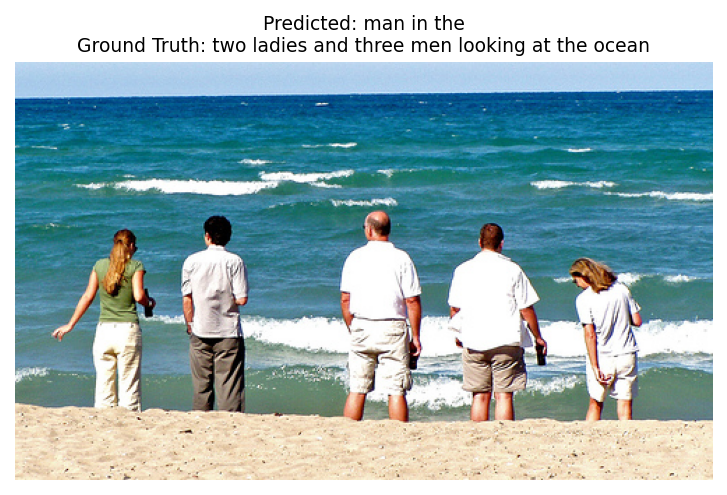
\includegraphics[width=0.8\textwidth]{selected_figures/baseline_example.png}
    \caption{Representative baseline output. The prediction is partially related to the scene but remains generic and incomplete with respect to the full reference description.}
    \label{fig:baseline_example}
\end{figure}

\begin{figure}[H]
    \centering
    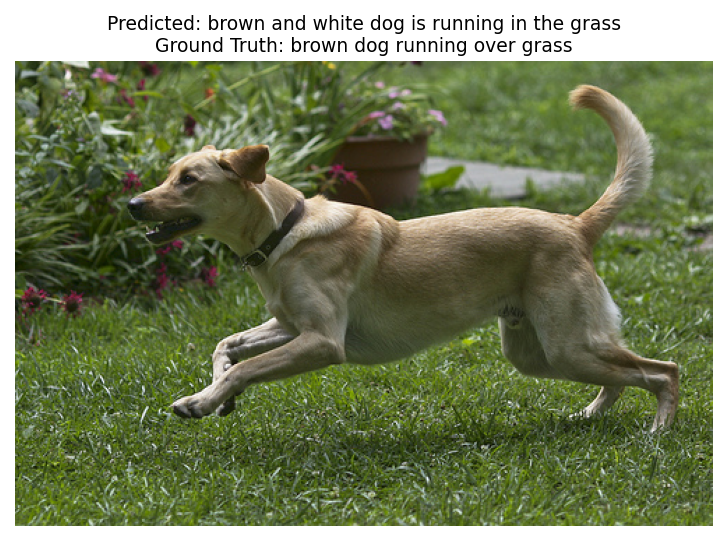
\includegraphics[width=0.8\textwidth]{selected_figures/finetune_example.png}
    \caption{Representative fine-tuned output. The generated caption correctly identifies the main object and action, and is more specific than the weaker baseline examples.}
    \label{fig:finetune_example}
\end{figure}

\begin{figure}[H]
    \centering
    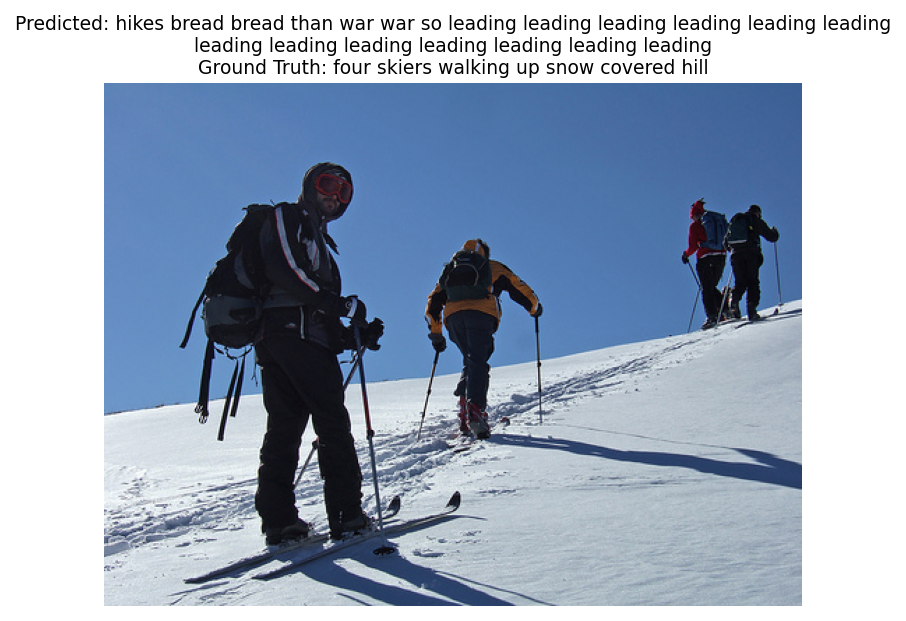
\includegraphics[width=0.8\textwidth]{selected_figures/failure_case.png}
    \caption{Failure case. The generated caption is repetitive and semantically incorrect, showing that the model may still collapse into unstable word sequences on difficult inputs.}
    \label{fig:failure_case}
\end{figure}

\section{Practical Constraints}

The project was developed and tested under CPU-only execution. This had three implications:
\begin{itemize}[leftmargin=*]
    \item training time was significantly longer than in a GPU setting;
    \item checkpointing and resume support became practically important;
    \item the experimental protocol had to be controlled and staged carefully to avoid wasting runtime.
\end{itemize}

This limitation does not invalidate the experiments, but it is important context for interpreting the scale and depth of the final campaign.

\section{Limitations}

\begin{itemize}[leftmargin=*]
    \item Flickr8k is relatively small for image captioning, limiting the expressiveness of the learned model.
    \item The project focuses on a classical CNN-LSTM architecture and does not compare against more modern transformer-based methods.
    \item Some generated captions remain generic or unstable, especially in difficult scenes.
\end{itemize}

\section{Conclusion}

This project implemented a complete CNN-LSTM image captioning pipeline on Flickr8k, including preprocessing, vocabulary generation, dataset preparation, training, evaluation, and qualitative analysis. The experiments show that both scheduled sampling and label smoothing improve BLEU performance relative to their corresponding ablations. The best overall configuration was the fine-tuned model, which achieved the highest BLEU scores among all tested setups. The repository now contains the code, checkpoints, logs, result files, and qualitative figures necessary for a complete academic submission.

\section*{Artifacts Available for Submission}

The following files support the final report:
\begin{itemize}[leftmargin=*]
    \item \texttt{results/metrics\_summary.csv}
    \item \texttt{results/experiment\_summary.csv}
    \item \texttt{results/*\_predictions.json}
    \item \texttt{logs/*}
    \item \texttt{figures/*}
    \item \texttt{LAB\_LOG.md}
\end{itemize}

\end{document}
